\section{Feature Description} %3.3

The area of the sea ice in the Arctic is deemed relevant to the following features. The content of carbon dioxide, the area of the ozone hole over the Arctic, the land and ocean temperature in northern hemisphere, the Max/Ave/Min temperature of North Slope Alaska, the rainfall in the Arctic, daylight of Arctic and the population of the world.

\begin{figure}[t]
\center
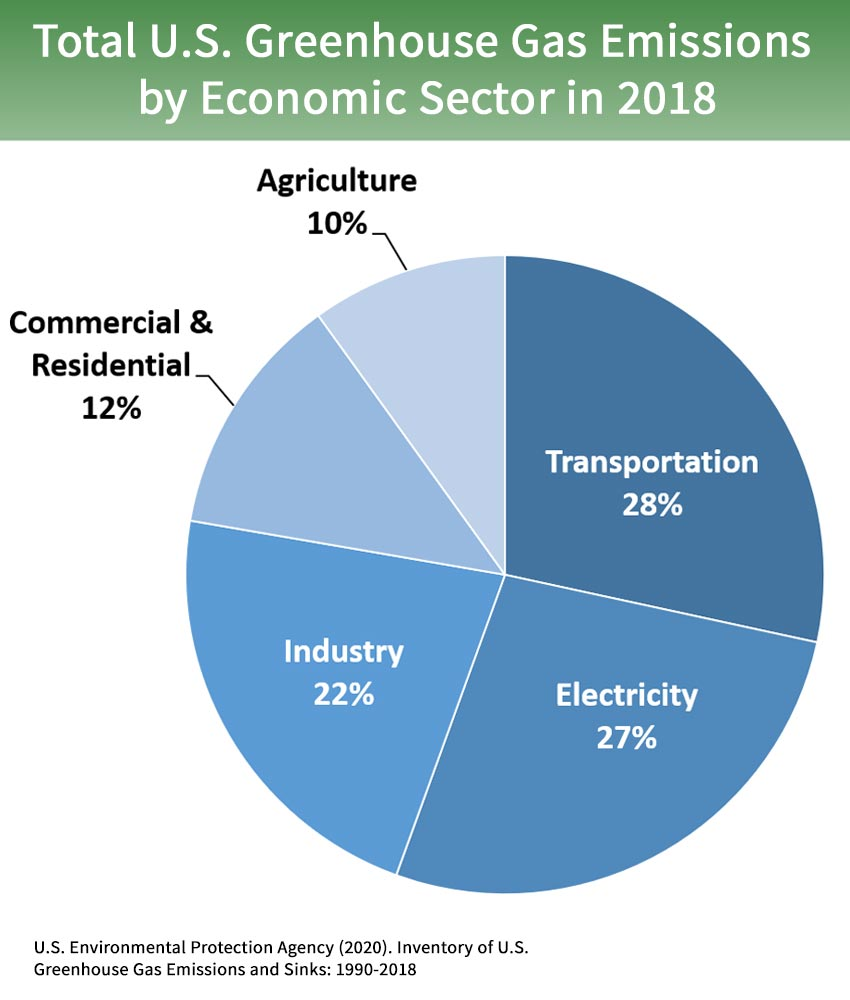
\includegraphics[width = 0.66\textwidth]{Figure/3.3-Overview-USGGE2018.jpg}
\longcaption{Total U.S. Greenhouse Gas Emissions by Economic Sector in 2018}{\label{3.3-Overview-USGGE2018} Total U.S. Greenhouse Gas Emissions by Economic Sector in 2018. Image courtesy: https://www.epa.gov/ghgemissions/sources-greenhouse-gas-emissions}
\end{figure}

Changes in the area of sea ice in the Arctic are believed to be related to the content of carbon dioxide. As shown in Figure \ref{3.3-Overview-USGGE2018}, Carbon dioxide accounts for 81 percentage of greenhouse gases. Thus the main component of greenhouse gases is carbon dioxide, which is also the main cause of the greenhouse effect. According to J.H.Mercer, the greenhouse effect will have a catastrophic impact on the ice sheets \cite{mercer1978west}. Thus the content of carbon dioxide is chosen to be one of the features.

In addition, according to the results of the common correlated effects mean group (CCEMG) estimator, the GDP growth and the population size influence CO2 emission levels positively and significantly, at both the global and regional levels \cite{DONG2018180}. In that case, the GDP growth and the population size would have impact on the ice sheets.

The ozone hole area is also considered to be related to the area of sea ice in the Arctic. In 2010, Sigmond and Fyfe found that the ozone depletion leads to a positive SAM response in austral summer, which induces sea ice melt \cite{sigmond2010has}. In that case, changes in the size of the ozone hole would also affect the changes in sea ice area. Thus the ozone hole area is chosen to be one of the features.

Furthermore, the temperature is deemed to be related to the area of sea ice in the Arctic. According to Ditlevsen and Grinsted's research, by considering a minimal model of an ice sheet, it shows that fluctuating temperatures have an effect on the mass balance and thus on the steady-state volume of the ice sheet \cite{mikkelsen2018influence}. Thus the temperature is considered to be a feature.

Changes in the area of sea ice in the Arctic are also believed to be related to the rainfall. According to Bromwich and Robasky, the increased precipitation may reduce the net loss of ice sheets area or even turn it into net gain \cite{Bromwich1993RecentPT}.Thus rainfall is considered to be a feature.


The amount of daylight in the Arctic is also believed to be related to the area of ice sheets. The Arctic has polar day and polar night phenomena, so there is periodicity in the phenomenon of daylight. As shown in Figure.....

% 这里添加一个光照周期的图,这边是光照的量还是光照的强度?然后这是真的找不到reference,最多就是说一下周期性,但是无法将光照和温度或者冰面扯上关系。


